\documentclass[11pt,a4paper]{article}
\usepackage[margin=2.2cm]{geometry}
\usepackage[T1]{fontenc}
\usepackage[utf8]{inputenc}
\usepackage{xcolor}
\usepackage{enumitem}
\usepackage{parskip}
\setlength{\parskip}{0.45em}
\usepackage{graphicx}
\usepackage{booktabs}
\usepackage{float}
\usepackage{hyperref}
\hypersetup{colorlinks=true,linkcolor=blue,urlcolor=blue}
\graphicspath{{figures/}}
\setlist[itemize]{leftmargin=1.5em}
\setlength{\emergencystretch}{2em}
\long\def\comment#1{\begin{quote}\small\itshape\noindent\textbf{Reviewer comment (full text).} #1\end{quote}}
\newcommand{\response}{\noindent\textbf{Response.} }
\newcommand{\change}[1]{\par\smallskip\noindent\textit{Revision in manuscript:} #1\par\medskip}

\title{Point-by-Point Response to the Editor and Reviewers}
\author{Zhi Huang, on behalf of all authors}
\date{19 July 2026}

\begin{document}
\maketitle

\noindent\textbf{Submission ID:} 56f53c41-a86e-4948-8cfd-a3c11b83fd1b

\noindent\textbf{Manuscript title:} BioInteract: Interpretable Drug--Target Interaction Prediction via Residue-Level Cross-Attention with Biological Prior Knowledge

\medskip
\noindent Dear Ms Agnihotri, Dr Zoete, and Reviewers,

\medskip
We thank the Editor and all three reviewers for their detailed and constructive
assessment.  The revision follows a conservative evidence-first approach.  We
retain the original Davis records, preprocessing, 70/10/20 ratios, and seed 42,
then add only reproducible diagnostic analyses that can be supported by the
available data.  In particular, we (i) audit duplicate sequences and full-length
target identity; (ii) add exact-sequence-grouped cold-target and
exact-sequence-grouped cold-both
evaluations; (iii) add leakage-aware drug-only, drug-promiscuity, target-only,
and label-shuffled controls; (iv) report performance by target-identity bins;
and (v) narrow all claims about generalisation, structural interpretation,
medicinal-chemistry utility, and resistance modelling.  We do not represent
unperformed external-dataset, structural-contact, or matched resistance
experiments as completed.

\paragraph{Revision-location guide.}
Page references below use the compiled clean manuscript dated 19 July 2026.
The Abstract and Introduction are on pp.~1--2; Related Work on pp.~2--3;
Methods on pp.~3--6; Experimental Setup on pp.~6--7; Results on pp.~7--14;
Discussion on pp.~15--16; Conclusion on p.~16; the web-server figure is on
p.~17; and availability statements are on p.~18. In the Supporting Information, model/training and environment details are
on pp.~1--2, split summaries are on p.~3, reproducibility details are on p.~4,
input/case/parameter audits are on pp.~5--6, and strict BindingDB provenance is
on p.~7. This guide supplements the section-level locations provided after each
response.

\section*{Response to the Editor}

\subsection*{E.1. Validation, overstatement, and manuscript/code reconciliation}

\comment{``The reviewers have identified substantial limitations. In particular,
the Methods and experimental evaluation should be strengthened by providing more
rigorous validation, including broader and fairer benchmarking, better
justification of dataset and baseline selection, more comprehensive ablation and
interpretability analyses, and appropriate controls for the reported claims. It
is also important to ensure that all conclusions are fully supported by the
presented evidence, address potential sources of bias and confounding factors,
and clarify any discrepancies between the manuscript and the accompanying
implementation.''}

\response We have addressed the parts that can be substantiated from the
submitted Davis material and have explicitly identified the remaining evidence
limits.  The revised manuscript now (i) adds exact-sequence grouping,
exact-sequence-grouped cold-target and exact-sequence-grouped cold-both tests;
(ii) quantifies
drug-side signal and target relatedness with controls and identity-stratified
  results; (iii) restores the numerical baseline comparison and component-removal
  ablation results; and (iv) redefines attention and Grad-CAM as
model-native attributions rather than structural contacts.  The web figure and
command-line statements now describe only functionality supported by the
repository and displayed screenshot.  We do not claim that the new within-Davis
controls replace external benchmarking, fair matched-encoder baselines, or
structural validation.

During final pre-submission reconciliation, we also found that the legacy
entity-split prediction CSVs and result JSON files could not be regenerated from
the released checkpoints, current inputs, and code. We therefore rebuilt the
three entity-split artifacts by instantiating each checkpoint from its embedded
configuration, collecting full-precision predictions, selecting each F1
threshold once on validation data, and applying that threshold unchanged to the
test data. The canonical artifact records hashes for checkpoints, data inputs,
cached embeddings, and model configurations; it now drives every reported
entity-split number, prediction CSV, bootstrap interval, and performance
figure. Figure~2 was redrawn from the reported component-removal results for
consistent presentation.

We also completed a final manuscript--code reconciliation and consistency audit:
\begin{itemize}
  \item Figure~3 now presents the canonical entity-split reconstruction as Panel
  A and the separately trained exact-sequence-grouped strict evaluations as
  Panel B; the identifier-based protocols are named ``Target-ID-held-out'' and
  ``Drug-ID-held-out'' consistently.
  \item The protein-side optional channel is named the ``domain-label channel''
  or, where its actual content matters, the ``unknown-label embedding channel.''
  We define ``biological prior knowledge'' as the frozen ESM-2 representation
  plus residue physicochemical features, not Pfam/InterPro annotation.
  \item The final checkpoint reconstruction uses each checkpoint's embedded
  architecture configuration, direct full-precision inference, and a
  validation-selected frozen threshold. The updated BioInteract values are used
  in the numerical baseline-comparison table and figure.
  \item Figure~2 now presents all reported component-removal rows and their
  AUROC changes in a legible two-panel layout.
  \item The attention-sparsity Methods now give the normalisation and sparsity
  equations, checkpoint, sample scope, and residue-pooling rule. The unused
  arbitrary ``hotspot'' definition has been removed.
  \item The Methods/SI now report the alignment function and scoring parameters,
  normalised-Indel implementation, non-chiral Morgan setting, exact software
  versions, ordinary pair-bootstrap procedure, seed and percentile interval,
  and the Grad-CAM layer and pre-sigmoid target.
\end{itemize}

\change{Abstract; Introduction; Related Work; Methods, ``Training Provenance and
Evaluation Thresholds'', ``Attention Sparsity'', ``Grad-CAM Functional-Group Attribution'',
and ``Data Splitting
Protocols and Similarity Audit''; Results, ``Comparison with Baseline Methods''
and ``Ablation Study''; Discussion;
Supporting Information Tables~S3--S7 and S13; Figs.~1--7 and captions.}

\subsection*{E.2. Archive code in a DOI-issuing repository}

\comment{``Please note that if your manuscript uses any custom or bespoke
computational tool or code, or reports a new algorithm, tool, software, or a
pipeline (even if individual components are not new), the underlying code must
be deposited in a recognised DOI-assigning repository (e.g. Zenodo) and linked
either from Methods or a dedicated Code Availability section.''}

\response We added a dedicated Code Availability section with direct links to
the public source repository, \url{https://github.com/Liubo-520/bio-intelligence},
and the immutable Zenodo software archive,
\url{https://doi.org/10.5281/zenodo.21437753}. The archive contains the released
code, pretrained weights, configuration files, canonical prediction CSVs,
provenance hashes, figure-generation scripts, strict BindingDB aggregate
manifests and audit, and reproduction instructions;
the Hugging Face Space provides the custom-prediction interface described in
the revised manuscript.

\change{New ``Code Availability'' section; Data Availability section.}

\section*{Response to Reviewer 1}

\subsection*{General assessment and strengths}

\comment{\textbf{General assessment}\par
The manuscript presents BioInteract, an interpretable DTI prediction framework
based on pharmacophore-aware molecular graphs, ESM-2 residue embeddings, domain
annotations, and bidirectional atom--residue cross-attention. The work is
technically interesting and the Davis benchmark results are encouraging,
especially in the cold-target setting.\par

However, the main claims remain stronger than the current evidence supports. The
model addresses a binary high-affinity classification task, whereas several
sections interpret attention and Grad-CAM outputs as direct evidence of binding
mechanisms. Additional controls are needed to distinguish genuine interaction
learning from ligand-side QSAR, target homology, and activity-profile biases.\par

\textbf{Strengths}\par
The architecture is well motivated and combines relevant molecular and protein
representations. The comparison includes random, cold-drug, and cold-target
splits, which is appropriate for this type of task. The manuscript is generally
clear, and the supplementary information provides useful implementation and
split details.}

\response We appreciate this balanced assessment. The revision directly follows
the distinction identified here: BioInteract is now described as a binary
high-affinity classifier on the Davis benchmark, while attention and Grad-CAM
are described as model-native attribution outputs rather than direct evidence of
binding mechanisms. The strict split audit, ligand-side controls, target-
relatedness analysis, and restricted case-study language address the stated
risks of QSAR, homology, and activity-profile bias in the sections detailed
below.

\change{Abstract; Introduction; Methods, \emph{Problem Formulation} and
\emph{Data Splitting Protocols and Similarity Audit}; Results; Discussion and
Conclusion.}

\subsection*{R1.1. Simpler QSAR and dataset-bias explanations}

\comment{\textbf{1. Simpler QSAR and dataset-bias explanations are not excluded.}\par

The ablation study does not sufficiently test whether BioInteract learns
drug--target interaction patterns, as opposed to ligand-side activity profiles
or matrix-completion effects. The \texttt{w/o ESM-2} model still receives target
information, and the \texttt{w/o cross-attention} model does not test how far a
simple ligand-only model can go.\par

This is important because, in the cold-target split, the proteins are unseen but
the ligands may already be present in training. The authors should include
diagnostic baselines, especially a simple drug-only multilabel QSAR model
predicting kinase activity profiles without protein input. Target-only,
degree/promiscuity-based, and shuffled-pair controls would also help determine
how much performance remains without explicit interaction modelling. If these
controls perform well, the claims about learned molecular-recognition principles
should be narrowed.}

\response We agree that the submitted ablation did not rule out drug-side
signal. A target-profile multilabel predictor cannot be evaluated for an unseen
target without introducing its held-out labels; we therefore use a pair-level,
drug-only Morgan logistic diagnostic that receives no target representation and
only training-partition labels. We also state explicitly that the label-shuffled
control is a label-sanity control rather than the requested structure-level
shuffled-pair experiment. We therefore added four leakage-aware diagnostic
controls to the same exact-sequence-grouped cold-target test (5,984 pairs; 208
positives). The
drug-only Morgan logistic control, which receives no target representation,
achieves AUROC/AUPRC of 0.764/0.164.  A drug-promiscuity prior estimated only
from training targets gives 0.764/0.163.  In contrast, the only target-only
control that is valid for unseen target identifiers is the uniform training
prevalence (0.500/0.035): using a held-out target's full label degree would
leak test labels.  A deterministic training-label-shuffled drug-only control
gives 0.407/0.029.  BioInteract achieves 0.873/0.383 on the same strict test.

These results show that ligand-side activity/promiscuity signal is material in
Davis.  BioInteract exceeds the diagnostic controls, but we do not interpret
the difference as proof of physical interaction learning or structural
recognition.  The manuscript now states this boundary explicitly.  We describe
the shuffled-label test accurately as a label-sanity control, not as a
structure-level shuffled-pair experiment.

\begin{table}[H]
\centering
\small
\caption{Evidence for R1.1: leakage-aware controls on the exact-sequence-grouped cold-target test.}
\begin{tabular}{lrr}
\toprule
Control or model & AUROC & AUPRC \\
\midrule
BioInteract (exact-sequence-grouped cold-target) & 0.873 & 0.383 \\
Drug-only Morgan logistic & 0.764 & 0.164 \\
Drug-promiscuity prior & 0.764 & 0.163 \\
Target-only constant prior & 0.500 & 0.035 \\
Label-shuffled drug-only & 0.407 & 0.029 \\
\bottomrule
\end{tabular}
\end{table}

\change{Methods, ``Data Splitting Protocols and Similarity Audit''; Results,
new Table ``Leakage-aware diagnostic controls'' and revised manuscript Fig.~4;
Discussion, new ``Diagnostic Controls and Remaining Dataset Bias''.}

\subsection*{R1.2. Control cold-target performance for target homology}

\comment{\textbf{2. Cold-target performance should be controlled for target homology.}\par

The cold-target result is strong, but its interpretation is currently too broad.
Davis contains kinase inhibitors and kinase targets, so a test target can be
absent from training while still being highly homologous to training kinases. The
result may therefore reflect transfer within the kinome more than generalisation
to biologically distant targets.\par

The authors should report the maximum sequence identity between each cold-target
test protein and the training targets, preferably for both full-length sequences
and kinase domains. A homology-reduced cold-target split, for example after
clustering targets at a defined identity threshold such as 60\%, would be
particularly informative. At minimum, performance should be stratified by
target-similarity bins.}

\response We added a full-length global-alignment audit for the
exact-sequence-grouped cold-target split.  For each of 88 held-out targets, we
report the maximum exact-residue identity divided by aligned length against all
310 training targets.  The maximum identity ranges from 0.231 to 0.867 (median
0.494).  The four identity bins contain 31, 28, 24, and 5 targets below 0.40,
0.40--<0.60, 0.60--<0.80, and at least 0.80, respectively.  Corresponding
pair-level BioInteract AUROC/AUPRC values are 0.806/0.305, 0.908/0.456,
0.908/0.466, and 0.862/0.121.  The final bin contains only three positives, so
its AUPRC is unstable.  These non-monotonic results make residual relatedness
visible but do not establish distant-family transfer.

We did not claim a kinase-domain-specific identity analysis or a 60\%-clustered
split because no independently curated kinase-domain boundaries or new split
results were supplied.  Instead, the manuscript now makes the full-length
analysis and its limitation explicit.

\begin{figure}[H]
\centering
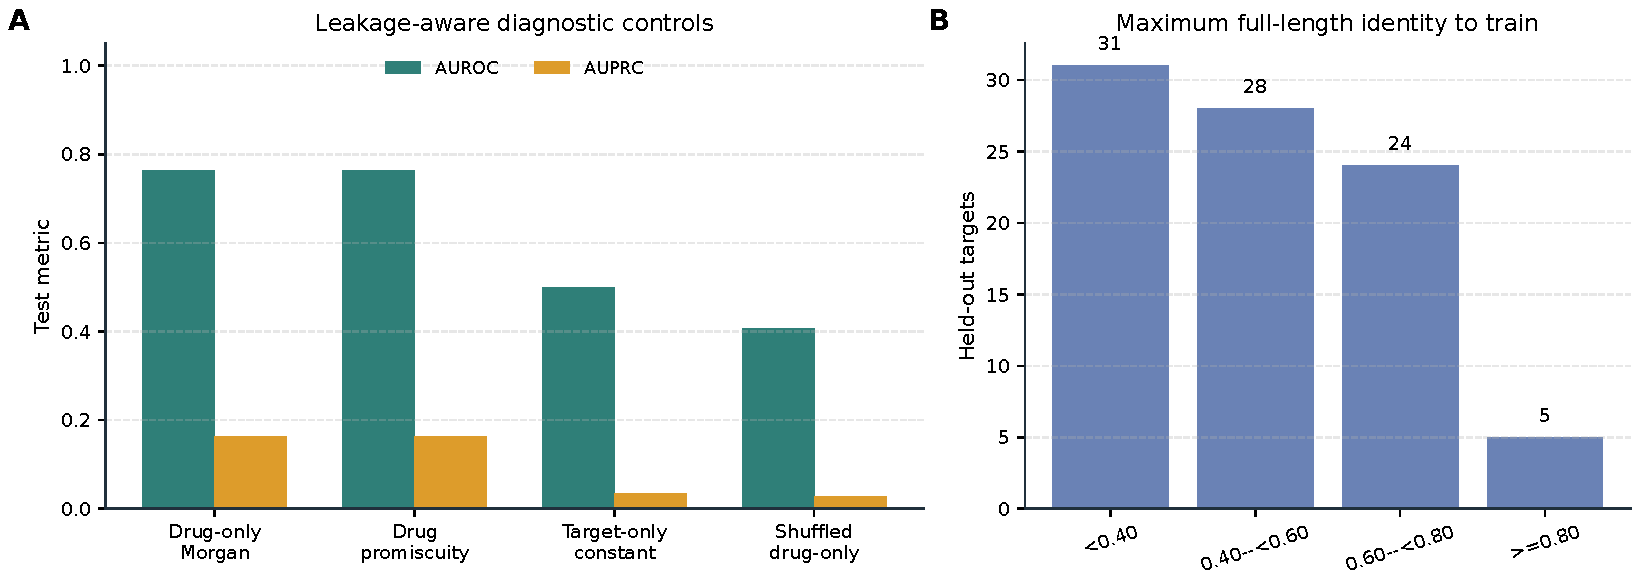
\includegraphics[width=0.92\linewidth]{figures/fig_reviewer_controls.pdf}
\caption{Evidence for R1.1--R1.2.  Panel A shows leakage-aware controls;
Panel B gives the count of exact-sequence-grouped cold-target test proteins by maximum
full-length identity to a training target.}
\label{fig:response_controls}
\end{figure}

\change{Methods, ``Data Splitting Protocols and Similarity Audit''; Results,
new diagnostic-control table and revised manuscript Fig.~4; Discussion,
``Scope of Cold-Start Evaluation''.}

\subsection*{R1.3. Resistance-mutant analysis}

\comment{\textbf{3. The resistance-mutant analysis does not yet show resistance-aware modelling.}\par

The ABL1 mutant examples mainly show conserved attention across selected mutant
cases that remain high-affinity binders. This supports attention stability across
similar positive cases, but it does not demonstrate that the model captures
resistance-associated loss of activity.\par

The authors should include matched WT/mutant examples for the same inhibitor
where the mutation experimentally reduces binding or activity. The model should
then show both a lower predicted binding probability and an interpretable shift
in the residue-level attention map. Without this analysis, the section should be
reframed as attention conservation across selected ABL1 binder cases.}

\response We thank the reviewer for prompting a closer audit of the actual Davis
model inputs. The nominal ABL1 wild-type, F317I, F317L, M351T, E255K, and
suffix-labelled records used here have identical 1,167-residue sequences and
the same SHA-256 digest in \texttt{target\_sequences.csv}. Thus the model never
receives a sequence change that corresponds to the nominal variant label. We
have removed the entire previous mutant-comparison analysis, including its
tables, figures, case study, and all resistance-related conclusions, rather
than reframe it as a stability result. The revised manuscript states this
limitation transparently, and Supporting Information Table~S9 records every
identifier, length, digest, and the associated D0010/D0017 Davis records.

\change{Results, ``Audit of Nominal ABL1 Variant Inputs''; Discussion,
``Limitation of Nominal ABL1 Variant Records''; Supporting Information,
Table~S9.}

\subsection*{R1.4. Validation of interpretability analyses}

\comment{\textbf{4. The interpretability analyses need stronger validation.}\par

The attention sparsity, Grad-CAM pharmacophore rankings, target-dependent
pharmacophore profiles, and hotspot-count analysis are interesting, but they
remain exploratory. Sparse attention does not by itself prove binding-pocket
localisation, and Grad-CAM agreement with general kinase-inhibitor SAR is not
sufficient mechanistic validation.\par

The authors should compare high-attention residues with experimentally resolved
ligand--protein contacts when structures are available. They should also clarify
how atom-level Grad-CAM scores are aggregated into functional groups and test
whether these profiles are stable across related ligands or matched analogues.
The BRAF example, which is a low-confidence false-negative case, should be
treated as a failure-mode analysis rather than as positive evidence for
target-dependent pharmacophore usage. The hotspot-count analysis should also be
softened, since it is based on few selected cases and an arbitrary attention
threshold.}

\response We agree that sparse attention and Grad-CAM are exploratory without
independent supervision.  The Methods now define functional-group values as
aggregated atom-level Grad-CAM attributions and state that they are neither
contacts nor interaction types.  The manuscript cites structurally supervised
work such as MONN to distinguish that setting from the present one.  No
PDB/PLIP contact comparison or matched-analogue stability test was performed,
and none is claimed.  The BRAF/D0023 result is now a low-confidence
failure-mode example, not positive evidence for target-dependent functional-group
usage.  We removed the hotspot-count analysis and figure because the selected
cases included nominal ABL1 variants with identical model-input sequences and
the arbitrary threshold could not support a structural or affinity claim.

For reproducibility, the revised Methods define residue score
$s_j=\sum_i M_{ij}$, pair-specific normalisation
$\widetilde{s}_j=s_j/\max_k s_k$, and
$\mathrm{Sparsity}=|\{j:\widetilde{s}_j<0.1\}|/L$. The reported 99.2\% value
uses \texttt{checkpoints/best.pt} and all 1,506 positive Davis pairs, including
original training, validation, and test memberships. Each pair is normalised
before pooling all 1,301,380 residue observations; consequently, longer proteins
contribute more residue-level observations. Grad-CAM is computed at the final
(third) GINE layer with respect to the pre-sigmoid interaction logit. No residue
is designated a biological hotspot.

\change{Related Work, ``Interpretability in DTI Models''; Methods,
``Grad-CAM Functional-Group Attribution''; Results, non-mutant
interpretability case studies; Discussion, ``Functional-Group Attribution
Without Structural Supervision''; removed former hotspot-count analysis and
figure.}

\subsection*{R1.5. Figure 2 readability}

\comment{\textbf{Minor comment: Figure 2 should be redrawn for readability,
especially the right panel.}}

\response We restored the component-removal numerical rows and redrew the figure
for readability. The revised Figure~2 now identifies Panels~A and B, separates
the metric heatmap from the AUROC-difference panel, moves the legend below the
bars, and uses non-overlapping labels. Panel~B now includes all four
component-removed rows, including graph augmentation, so the figure and Table~2
carry the same information.

\change{Results, ``Ablation Study''; Table~2 and Figure~2.}

\subsection*{R1.6. Training dynamics and overfitting}

\comment{\textbf{Minor comment:} Section 5.4 should avoid stating that the
training curves confirm absence of overfitting. Validation AUPRC, validation
loss, and repeated-seed variability would make this point more convincing.}

\response We agree. We removed the assertion that single-seed training curves
confirm absence of overfitting. Following final log audit, Figure~5 was rebuilt
from one contiguous trace per protocol whose peak validation AUROC matches its
saved checkpoint; duplicated and restarted log segments were excluded. The
revised text limits the figure to observed validation-AUROC and training-loss
trajectories and explicitly states that they do not quantify validation loss or
repeated-seed variability.

\change{Results, ``Training Dynamics'' and Figure~5 caption.}

\subsection*{R1.7. Binary classification and cautious cold-drug interpretation}

\comment{\textbf{Minor comments}\par
The manuscript should consistently distinguish binary high-affinity
classification from quantitative affinity prediction. Claims related to
potency, lead optimisation, and mechanistic binding should be moderated
accordingly.\par

The cold-drug results should be discussed more cautiously. BioInteract improves
over the selected baselines, but the absolute AUPRC and thresholded metrics
indicate limited generalisation to unseen molecules.}

\response We revised the Introduction, Methods, Results, Discussion, and
Conclusion to define the task as binary classification of Davis pairs at
$K_d<30$ nM.  We removed potency, lead-optimisation, and ranking language from
the present results.  Continuous affinity prediction is stated only as future
work. We also clarify that Drug-ID-held-out means unseen identifiers, not validated
scaffold hopping or out-of-distribution chemical generalisation; its AUPRC and
thresholded metrics are interpreted cautiously.

\change{Abstract; Introduction; Methods, ``Problem Formulation'' and
``Evaluation Metrics''; Results, Drug-ID-held-out discussion; Discussion and
Conclusion.}

\subsection*{Reviewer 1 recommendation}

\comment{\textbf{Recommendation: Major revision.}\par
The study is promising, but the central claims require stronger diagnostic
controls and more cautious interpretation. The key revisions are a ligand-only
QSAR control, a homology-aware cold-target evaluation, a more informative
resistance-mutant analysis, and structural or SAR-based validation of the
interpretability outputs.}

\response We appreciate this clear recommendation. The added ligand-only and
promiscuity controls, exact-sequence-grouped cold-target evaluation, and
full-length identity stratification directly address the first two requests. As
the nominal ABL1 variants have identical model-input sequences, the mutant
analysis was withdrawn in full. Because matched loss-of-activity and
structural-contact data were not available, the remaining non-mutant attribution
analyses are explicitly presented as exploratory model behaviour rather than
validated mechanistic findings.

\change{Results and Discussion revisions identified in R1.1--R1.7.}

\section*{Response to Reviewer 2}

\subsection*{R2.1. Methodological novelty}

\comment{\textbf{1.} The combination of ESM-based protein representations and
graph-based molecular encoders, often together with attention-based interaction
modules, is not entirely new in DTI/DTA prediction. Therefore, the manuscript
should more clearly clarify the methodological novelty of the proposed framework
compared with existing ESM + graph encoder models and their attention-based
extensions.\par
1) PGraphDTA: Improving Drug Target Interaction Prediction using Protein Language
Models and Contact Maps\par
2) HCAF-DTA: drug-target binding affinity prediction with cross-attention fused
hypergraph neural networks\par
3) GEFA: Early Fusion Approach in Drug-Target Affinity Prediction\par
etc.}

\response We agree that these individual ingredients are not new. The revised
Related Work now explicitly cites GEFA, PGraphDTA, and HCAF-DTA and states that
BioInteract does not claim first use of a protein language model, a graph
encoder, or cross-attention in DTI/DTA prediction. We have narrowed the claimed
contribution to the submitted integration of chemistry-aware molecular graphs,
residue-level ESM-2/physicochemical features with a configured unknown-label
embedding channel, and model-native attribution outputs for Davis binary
classification. The new text also cites 3DProtDTA, the domain-specific framework
of Liu \textit{et al.}, and InceptionDTA when discussing the broader
multi-benchmark DTA literature requested by the reviewers. These citations are
used to situate the scope and do not imply a direct numerical comparison across
different task definitions, label transformations, data processing, or splits.
Finally, we clarify throughout that the attribution outputs are not independently
validated structural evidence.

\change{Related Work, ``Pretrained Protein Language Models'' and
``Interpretability in DTI Models''; Introduction and Conclusion.}

\subsection*{R2.2. Fair comparison with pretrained protein representations}

\comment{\textbf{2.} The cold-start comparison may not be entirely fair because
BioInteract uses frozen ESM-2 embeddings pretrained on a large-scale protein
sequence corpus, whereas the baseline models included in the manuscript do not
appear to use comparable pretrained protein representations. Therefore, the
reported improvement, especially under the cold-target split, may largely reflect
the benefit of ESM-2 pretraining rather than the proposed architecture itself.
The authors should include stronger baselines that also use pretrained protein
representations, such as ESM-based DTI/DTA models, or provide controlled
comparisons where the same pretrained protein features are used across competing
architectures.}

\response We agree that the baseline comparison does not isolate the effect of
ESM-2 pretraining. We restored the numerical baseline comparison but revised its
interpretation: it is presented as Davis benchmark context, not as controlled
evidence that the cross-attention architecture alone produces the observed
differences. The current reconstructed BioInteract entity-split values are used
in Table~1 and Figure~1, and the text explicitly states that no matched
ESM-based baseline was newly evaluated.

\change{Results, ``Comparison with Baseline Methods'' and ``Ablation Study'';
Tables~1--2; Figures~1--2; Discussion.}

\subsection*{R2.3. Davis-only evaluation and dataset bias}

\comment{\textbf{3.} The Davis dataset is highly kinase-specific and is known to
have strong dataset bias. Evaluating the model only on this dataset makes it
difficult to objectively assess its general DTI prediction performance. I
recommend additional evaluation on larger and more diverse datasets, such as
BindingDB, which contains a broader range of proteins and drug--target
interactions.}

\response We agree and added a pre-specified frozen external evaluation using
the official BindingDB curated-articles snapshot
\texttt{BindingDB\_BindingDB\_Articles\_202607}. We retained only exact,
finite $K_d$ measurements, used the same $K_d<30$~nM label definition,
excluded invalid or multi-chain records, and then excluded every ligand whose canonical isomeric SMILES or target
whose full normalised sequence occurred anywhere in Davis. The final strict
double-novel cohort contains 1{,}932 pairs (516 positive and 1{,}416 negative)
from 1{,}195 ligands and 396 targets.

For complete curation accounting, the sequential row-level filters leave 2{,}158
eligible measurements. The 15 threshold-conflicting ligand--target groups are
counted at the pair level and comprise 44 measurement rows; 2{,}114
threshold-consistent rows remain. For each consistent pair, we retain the median
exact $K_d$; 182 repeated measurement rows across 143 retained pairs are thereby
collapsed, yielding 1{,}932 final pairs. This procedure is now specified in the
Methods and Table~S13.

The released \texttt{best\_random} checkpoint was evaluated without retraining,
fine-tuning, recalibration, checkpoint selection, or threshold tuning on
BindingDB. At the frozen Davis random-validation threshold, it obtained AUROC
$=0.560$ (95\% CI 0.531--0.589) and AUPRC $=0.340$ (95\% CI 0.314--0.372);
F1, precision, and recall were 0.070, 0.731, and 0.037. The result does not support a broad DTI-transfer claim.
Rather, it documents limited transfer of the frozen Davis-trained classifier to
this broader exact-entity cohort. It leaves the within-Davis
checkpoint reconstructions unchanged and is not used as evidence for the
attention, attribution, structural, or mechanistic analyses.

\change{Methods, ``Pre-specified External BindingDB Evaluation''; Results,
``Strict External BindingDB Evaluation'' and Table~5; Supporting Information,
Table~S13; Discussion and Conclusion.}

\subsection*{R2.4. Baseline selection and recency}

\comment{\textbf{4.} The baseline selection also appears somewhat limited and
outdated. Among the compared methods, the most recent baseline appears to be
DrugBAN, which is marked as a 2023 model in the manuscript. Since more recent
DTI/DTA models have been proposed after 2023, including models using graph-based
molecular encoders, attention-based fusion, and pretrained protein
representations, the authors should include stronger and more up-to-date
baselines.}

\response We now cite verified examples of recent PLM, graph, and attention
models. We restored the original numerical comparison, but it is presented as
benchmark context rather than a current state-of-the-art leaderboard or a
controlled architecture comparison. We do not claim to have reproduced
additional baselines without matching their task definition, preprocessing, and
pretraining. A fair comparison requires a common protocol and matched pretrained
target features, which remain outside the evidence available in this revision.

\change{Related Work; Results, ``Comparison with Baseline Methods'';
Discussion, ``Future Directions''.}

\subsection*{R2.5. Biological meaning of attention maps}

\comment{\textbf{5.} The attention map represents the degree to which the model
attends to protein residues or drug atoms. However, Figure 5 alone is
insufficient to conclude that the model has truly identified biologically
meaningful interaction regions. Previous studies such as BlendNet and MONN
validated attention maps or pairwise interaction prediction maps using tools
such as PLIP to compare predicted interaction regions with actual protein--ligand
contacts. A similar validation would be necessary to support the interpretability
claim.\par
1) Exploring the potential of compound--protein complex structure-free models in
virtual screening using BlendNet\par
2) MONN: A Multi-objective Neural Network for Predicting Compound-Protein
Interactions and Affinities}

\response We agree.  We removed language that treated attention maps as
identified biological interaction regions.  The revised text distinguishes the
present unsupervised attribution output from models trained or evaluated with
explicit non-covalent interaction labels.  We did not run PLIP/PDBBind or
BlendNet/MONN-style structural validation, so the response and manuscript state
that a non-overlapping structural benchmark and defined contact protocol are
required before assigning structural meaning.

\change{Related Work, ``Interpretability in DTI Models''; Results,
``Case Study: Functional-Group Attribution'' and ``Cross-Case Functional-Group
Attribution Variation''; Discussion, ``Functional-Group Attribution Without
Structural Supervision'' and ``Future Directions''.}

\subsection*{R2.6. Mutation-pattern analysis}

\comment{\textbf{6.} It is unclear why analyzing mutation patterns is important for
this model. If the goal is to demonstrate interpretability, simply analyzing
residues with high attention scores is not sufficient. More detailed biological
or structural analysis is needed to show that the model captures meaningful
mechanisms rather than merely producing attention weights.}

\response We agree. A direct audit showed that all nominal ABL1 variant inputs
used by the model have an identical amino-acid sequence. We therefore removed
the former mutation-pattern analysis in full and do not use it as evidence of a
biological mechanism. The revised Results and Discussion state that these Davis
records cannot support a mutation-effect or resistance analysis for BioInteract;
the reproducible input audit is supplied in Table~S9.

\change{Results, ``Audit of Nominal ABL1 Variant Inputs''; Discussion,
``Limitation of Nominal ABL1 Variant Records''; Supporting Information,
Table~S9.}

\subsection*{R2.7. Remaining case studies}

\comment{\textbf{7.} The remaining case studies would be more convincing only after
the model has been validated on larger and more diverse datasets. Based on the
current results, it is difficult to determine whether the proposed model truly
provides reliable interpretability or mechanistic insight.}

\response We agree that the cases are illustrative rather than validation. The
new BindingDB test supplies a strict external performance check, but its limited
transfer result is not evidence for case-level interpretability or mechanism.
All case-study language therefore describes observed model behaviour or a
failure-mode example, and the Conclusion does not use the cases to establish a
mechanistic conclusion. Structural validation remains necessary.

\change{Results, ``Strict External BindingDB Evaluation'' and all interpretability
case studies; Discussion; Conclusion.}

\subsection*{Reviewer 2 overall assessment}

\comment{Overall, while the proposed model is interesting, the current manuscript
would benefit from clearer novelty claims, fairer baseline comparisons,
evaluation on larger-scale datasets, and more rigorous validation of the
interpretability results.}

\response We agree with these priorities. The revision adds a strict external
BindingDB evaluation, reports its limited transfer transparently, narrows the
novelty claim, labels baseline comparison limitations, and removes structural or
mechanistic interpretation claims that are not independently validated.

\change{Related Work; Methods, external evaluation; Results, baseline comparison,
split audit, and external test; Discussion; Conclusion.}

\section*{Response to Reviewer 3}

\subsection*{R3.0. General comment: website and command-line accessibility}

\comment{\textbf{General comments.}\par

Although this work appears to be comprehensive, scientifically accurate, and
technically sound, the authors should be careful to not overstate the
capabilities of their framework, given the limitations of their dataset and the
lack of explicit structural cross-validation (see questions below).\par

The authors have provided a codebase that is maintained on GitHub, facilitating
the reproducibility of the findings and data analysis performed in this paper.
However, the publicly accessible huggingface.co website does not appear to work
properly for a couple of the pre-computed case studies (BRAF + Drug 11717001
(Sorafenib analogue) and EGFR + Drug 156414). Namely, the Top Predicted Binding
Residues and Pharmacophore Group Importance (Grad-CAM) plots are not displayed
for these case studies, nor are the predicted binding probability, model
confidence, or experimental affinity shown. These plots also seem to be missing
from the corresponding GitHub folder (the \texttt{hf\_space} subfolder) in the repository,
although Grad-CAM molecule figures seem to be available for 156414-EGFR and
11717001-BRAF (inside the results/interpretability/gradcam/ folder in the
repository). Reassuringly, the Custom Prediction tab appears to be working for a
user-provided drug SMILES and protein amino acid sequence. The authors appear to
omit some of the functionality provided in their repository codebase within
their publicly available huggingface.co space, and it is not clear why some
features appear to be available within the code but not described within the
context of the manuscript (see questions below). It would be useful if the
authors could provide instructions on how to utilize the functionality of their
GitHub repository to make predictions and generate outputs for custom ligands
and targets through command-line operation, which would greatly increase the
accessibility of the code and allow the larger scientific community to utilize
the resource without having to input potentially proprietary information into a
web server.}

\response We agree that the browser demonstration and the repository must not
be conflated. Figure~7 is described as the
custom-prediction input/result state shown for human Aurora kinase C (UniProt
Q9UQB9), including the generated atom--residue attention map and ``Top 10
Residue Attributions'' chart visible in the lower portion of the screenshot.
These are identified as model-native attribution views, not a residue-contact
map, hotspot label, or experimental affinity. We do not use the displayed web
case as evidence for the manuscript's scientific claims.

For reproducibility, the revised Code Availability text directs readers to the
repository README and identifies the supplied commands for training, evaluation,
and archived-case attribution:
\begin{quote}\footnotesize\ttfamily
python -m src.cli.train\\
\quad -{}-config configs/default.yaml\\
python -m src.cli.evaluate\\
\quad -{}-config configs/default.yaml -{}-checkpoint checkpoints/best.pt\\
python -m src.cli.interpret\\
\quad -{}-config configs/default.yaml -{}-checkpoint checkpoints/best.pt
\end{quote}
The current command-line interface does not constitute a
general structure-based custom-ligand/pocket workflow, and no such functionality
is claimed. This separates browser custom prediction from repository-based
evaluation and attribution generation.

\change{Data Availability; Figure~7 caption; Conclusion.}

\subsection*{R3.1. Rationale for Davis only and external validation}

\comment{\textbf{1.} Can the authors comment further on their rationale for
only choosing the Davis kinase inhibitor dataset to showcase the functionality
of BioInteract? Was this done solely to facilitate comparison to existing
drug-target interaction (DTI) software? By their own admission, this dataset is
highly imbalanced (5\% positive rate) and narrowly focused, comprising only 68
kinase inhibitor drugs and 442 protein kinase targets. Would the predictive
ability of the model against diverse binding pockets and out-of-distribution
chemical space not have been better showcased with a different dataset, such as
BindingDB or KIBA (as mentioned in Section 6.6 -- Future Directions), especially
considering that the authors chose to combine ESM-2 embeddings with Pfam/InterPro
domain information in their architecture? As it is currently presented, it is
difficult to validate the claim that the BioInteract architecture is designed to
be protein-family agnostic (which appears reasonable in theory) based only on
the results obtained from the Davis dataset. A quick survey of other papers in
the literature (e.g., doi: 10.1039/d3ra00281k, 10.1021/acs.jcim.4c00403,
10.1016/j.heliyon.2025.e42476) also shows that other authors usually evaluate
their model on multiple datasets in addition to the Davis dataset, including the
KIBA, BindingDB, BIOSNAP, and PDBBind datasets. While the authors mention
analyses on other datasets as a direction for future research, they are still
strongly encouraged to demonstrate the functionality of their model on at least
one other such dataset, both to bring their work in line with others in the
literature and to better assess the ability of their model.}

\response We agree that Davis-only evidence cannot establish broad protein-family,
binding-pocket, or chemical-space generalisation. Davis was retained because it
is the original submitted benchmark;
it was not selected as a demonstration of protein-family-agnostic performance.
All such language has been removed. We now add a pre-specified frozen BindingDB
external evaluation rather than treating the within-Davis controls as external
validation. The official curated-articles snapshot was filtered to exact finite
$K_d$ measurements and strict double novelty against all Davis ligands and full
target sequences. The sequential row-level filters leave 2{,}158 eligible
measurements. The 15 threshold-conflicting groups are pair-level counts and
comprise 44 measurement rows; the 2{,}114 remaining rows are aggregated by the
within-pair median exact $K_d$, collapsing 182 repeated rows to the final 1{,}932
pairs (516 positive and 1{,}416 negative). Without retraining, recalibration, or BindingDB threshold
tuning, the released \texttt{best\_random} checkpoint produced AUROC $=0.560$
(95\% CI 0.531--0.589) and AUPRC $=0.340$ (95\% CI 0.314--0.372). The result does not support a broad DTI-transfer claim.
It instead documents limited transfer to a broader exact-entity cohort and is
not used to support claims about binding pockets, attention maps, or
protein-family-agnostic performance.

During final reproducibility auditing, we also found that the released package
contains no per-protein domain-annotation JSON files. The archived loader assigns
its \texttt{NONE} domain label when such a file is absent, so the released Davis
inputs do not provide curated Pfam/InterPro annotations. We revised the abstract,
Methods, ablation interpretation, and Supporting Information to describe a
configured unknown-label embedding channel rather than a domain-enriched biological
 input. This correction avoids attributing either performance or interpretability
 to annotations that are not present in the reproducible assets.

We also added the three literature examples named in this comment---3DProtDTA,
the domain-specific DTI framework of Liu \textit{et al.}, and InceptionDTA---to
the Related Work. They provide appropriate context for the reviewer\'s request
because they use broader benchmark coverage, but we do not present their reported
scores as direct baselines: their endpoints, label definitions, preprocessing,
and training protocols are not matched to the Davis binary-classification setup.
The strict frozen-checkpoint BindingDB result is therefore retained as the
external evidence for this revision, with its limited transfer stated plainly.

\change{Methods, ``Pre-specified External BindingDB Evaluation'' and ``Configured
Domain-Label Channel and Availability''; Results, external evaluation and
ablation interpretation; Supporting Information, Table~S13; Discussion and
Conclusion.}

\subsection*{R3.2. Cold-drug/cold-target definitions, similarity, and redundancy}

\comment{\textbf{2.} Can the authors elaborate further on the splitting method
for their Cold-drug split and Cold-target split protocols? What is the Tanimoto
similarity between the drugs in the training and testing sets for the Cold-drug
split? Can the authors provide a pairwise similarity matrix or, for example, a
t-SNE projection of the Morgan fingerprints of both sets? How do the authors
define structurally novel molecules in this regard? Similarly, for the
Cold-target split, what is the maximum sequence similarity of the test set
proteins relative to the training set? It is extremely difficult to obtain
proteins that are truly sequentially novel as the authors claim. From other
publications (e.g., doi: 10.1016/j.heliyon.2025.e42476), it appears that the
Davis dataset may contain up to 15\% redundant protein sequences resulting from
multiple identifiers per sequence. It is not evident that the authors have
accounted for this fact.}

\response We define the original Drug-ID-held-out protocol as drug-identifier exclusion, not a scaffold
threshold or a claim of structural novelty. Radius-2, 1024-bit Morgan
fingerprints were generated without chirality and give maximum test-to-training Tanimoto values of 0.196--0.538
(median 0.257) for the 13 held-out drugs. We report this reproducible
test-to-training summary rather than presenting a t-SNE projection or a
pairwise-similarity matrix as a definition of novelty.

For the original Target-ID-held-out split, the maximum RapidFuzz normalised Indel similarities range
from 0.382 to 1.000 (median 0.579), and the audit finds 18 duplicate-sequence
groups involving 81 target identifiers, with six groups crossing the original
train/test boundary. We label that protocol Target-ID-held-out and additionally
provide the stricter full-length global-identity audit in R1.2.

\change{Methods, ``Data Splitting Protocols and Similarity Audit''; Results,
split-audit text and Fig.~4.}

\subsection*{R3.3. Cold-both evaluation}

\comment{\textbf{3.} Related to Question 2, it appears that the authors have
written code for the ability to perform a Cold-both split (inside
\texttt{src/data/split.py}), in which neither ligand nor protein have been seen
in the training data. As written in the comment of the function in the codebase,
this is a true test of generalizability, and such functionality is essential for
cases in which both the target and the molecules that could bind the target are
unknown. Why do the authors choose to omit the description of this splitting
approach in the main text, and why do they not report any comparative metrics
using this splitting method? Such results could potentially augment the findings
of the manuscript and provide a stronger case for the true power of the
BioInteract attention framework.}

\response We agree that the omission was not justified. We now report an
exact-sequence-grouped cold-both test using the original records, preprocessing,
architecture, and seed. Unlike the historical identifier-split reconstructions,
each strict-split model was trained from initialisation on its corresponding new
training partition. Both use weighted BCE with 0.05 label smoothing, AdamW
($10^{-4}$ learning rate; $10^{-5}$ weight decay), batch size 64, five-epoch
warm-up plus cosine decay, and validation-AUROC selection with patience 15.
The complete artifact paths, SHA-256 hashes, selected epochs, and frozen
validation thresholds are reported in Supporting Information Table~S3. The
70/10/20 ratios are applied independently to drug
identifiers and exact target-sequence groups; only pairs in the corresponding
train--train, validation--validation, and test--test blocks are retained. This
produces 15,190/264/1,144 train/validation/test pairs and excludes 13,458
cross-block pairs, so 70/10/20 is not a pair-level proportion for this protocol.
Exact-sequence-grouped cold-target gives 0.873/0.383 AUROC/AUPRC;
exact-sequence-grouped cold-both gives
0.552/0.038 with 38 positive test pairs. The cold-both validation block has only
10 positives, and at its validation-selected threshold (0.936), test F1,
precision, and recall are all 0.000. Both protocols are labelled within-Davis
stress tests rather than proof of broad generalisation.

\begin{table}[H]
\centering
\small
\caption{Evidence for R3.3: exact-sequence-grouped cold-start evaluations.}
\begin{tabular}{lrrrrrr}
\toprule
Protocol & Test pairs & Positives & AUROC & AUPRC & F1 & Recall \\
\midrule
Exact-sequence-grouped cold-target & 5,984 & 208 & 0.873 & 0.383 & 0.468 & 0.428 \\
Exact-sequence-grouped cold-both & 1,144 & 38 & 0.552 & 0.038 & 0.000 & 0.000 \\
\bottomrule
\end{tabular}
\end{table}

\begin{figure}[H]
\centering

\includegraphics[width=0.92\linewidth]{figures/fig2_performance.pdf}
\caption{Evidence for R3.3: canonical current-release identifier-based splits
(Panel A) and added exact-sequence-grouped strict splits (Panel B).}
\end{figure}

\change{Methods, split protocols; Results, Table ``Strict within-Davis
cold-start evaluation'' and revised Fig.~3.}

\subsection*{R3.4. Scope of interpretation and medicinal-chemistry claims}

\comment{\textbf{4.} The authors make strong claims about the scientific insight
gained by the BioInteract model, claiming in Section 6.1 that a medicinal
chemist can use BioInteract not only to rank candidates but also to identify
critical functional groups, map binding pockets, and assess potential resistance
liabilities. However, the model does not provide any structural output, nor
does it compute any binding scores or energies for ranking purposes. Moreover,
there does not appear to be any way to directly visualize a labeled
2D-representation of the molecule (i.e., with atom labels to identify which
atoms are predicted to interact), see the predicted binding pose of a putative
small molecule binder in the binding pocket of the target protein (although
functionality appears to exist inside \texttt{src/interpret/visualize.py} in the
repository to generate a PyMOL visualization script), or simultaneously rank a
large library of molecules against a target by a quantitative metric (as would be
done in a virtual screen). Such functionality appears to fall outside the scope
of the model. Structure-based design is a hallmark of medicinal chemistry and
virtual screening approaches, and it is not directly addressed by this model.
Although useful quantitative plots are provided through the residue interaction
heatmaps and Grad-CAM scores, it is furthermore not clear how users can generate
Grad-CAM molecule heatmaps through the huggingface.co website, or through the
command line, as the authors have shown in Figure 9A. The authors point out that
residue-level mechanistic explanations are furnished, but in reality, even
residue-level is too coarse-grained when it comes to molecular interactions.
Which atoms of the residue are interacting with which atoms of the ligand? Is it
a residue sidechain interaction, or a residue backbone interaction? Is there a
pi-stacking interaction, cation-pi interaction, van der Waals contact, H-bond,
or polar interaction occurring with the ligand, and if so, which atoms of the
protein residue are involved? Are any residues acting as H-bond donors or
acceptors, and if so, which atoms of those residues are involved in the
interaction? What is the environment of the binding pocket? These are the kinds
of structure-based mechanistic explanations that drive medicinal chemistry and
drug discovery campaigns. The authors should try to rephrase their language in
the text to avoid making claims that are not fully supported by their approach,
especially when they acknowledge in their Future Directions (Section 6.6) that
direct structural validation is missing and would provide quantitative support
for interpretability claims.}

\response We agree. Attention matrices and Grad-CAM are now called
model-native attributions. We removed claims of binding-pocket mapping,
interaction typing, atom--atom contacts, pose prediction, energy calculation,
large-library ranking, and treatment-resistance assessment. The revised Grad-CAM text defines functional-group aggregation from
atom-level attribution and reports saved non-mutant EGFR/BRAF summaries in the
two functional-group attribution tables in Results; it does not present an
atom-contact or pose figure.

The repository README is identified as the route to the available training,
evaluation, and archived-case attribution workflows. We do not claim that the
present command-line interface provides a general custom-ligand Grad-CAM,
PyMOL-pose, or structure-based interaction workflow. Those functions would
require a separately validated structural protocol and are explicitly outside
the scope of the present binary classifier.

\change{Abstract; Methods; Results, functional-group attribution tables;
Discussion; revised web-interface figure and caption.}

\subsection*{R3.5. Attention sparsity and BRAF failure mode}

\comment{\textbf{5.} The authors' reported observation regarding attention
sparsity (Section 5.5.1 and 6.2), combined with the interesting failure mode
reported for D0023 and BRAF (Section 5.8 and Fig. 10), raises an intriguing
question about the training of BioInteract and the dataset used in this work. As
the authors note, D0023 does not make strong H-bonding interactions, but rather
interactions involving its aromatic ring, and has a low-confidence prediction
despite its sub-nanomolar experimental binding affinity. How do we know that the
model has not simply learned to associate H-bonding interactions to canonical
kinase hinge-region residues as a predictor of binding affinity? As the authors
themselves note in Section 6.3, the learned cross-attention patterns transfer
via conserved binding-site geometry, implying that the cross-attention module
would also be implicated in attending to molecules which do not make such
canonical geometric interactions. Instead of classifying this as an
out-of-distribution example, would this not rather fall under the category of a
few-shot example that the model did not handle accurately due to dataset
imbalances that influenced its attention mechanism? In this sense, can the
authors also comment on the possibility that attention sparsity, rather than
being an emergent property of the model, arises due to the limited and imbalanced
nature of the training data itself?}

\response We agree that no single explanation is supported by the available
analysis.  The 99.2\% value is now described only as a thresholded attribution
concentration statistic that may reflect learned regularities, class imbalance,
data composition, or their combination.  BRAF/D0023 is now labelled a
low-confidence failure-mode example.  We do not attribute it specifically to
out-of-distribution status, few-shot coverage, hydrogen-bond bias, or sparsity.

\change{Results, attention-sparsity and functional-group sections; Discussion,
``The 99.2\% Attention Sparsity''; Figure~6 and functional-group tables.}

\subsection*{R3.6. Scalability and implementation version}

\comment{\textbf{6.} Can the authors comment on the scalability of their model
with larger datasets? Even with the current Davis dataset, containing only 68
unique drugs, the model comprises over 2.4 million trainable parameters, the
majority originating from the 3-layer GINE drug encoder module. With a larger
dataset, such as BindingDB, containing more than 1 million unique molecular
entries, how feasible would it be to train the model? It seems like the training
process only uses a single NVIDIA GPU, but this computational overhead would not
necessarily be expected to scale linearly with data size. Also, for
reproducibility, could the authors mention which version of Python was used in
their implementation details? Although the requirements.txt file in the GitHub
repository suggests that Python >= 3.8 was used, the authors do not explicitly
state the version that they used in the text.}

\response The Methods now state Python 3.10.14, PyTorch/PyTorch Geometric,
automatic mixed precision, and single-NVIDIA-GPU training.  The model has
2,442,083 trainable parameters.  We do not claim linear scalability to
BindingDB-scale data; larger datasets require profiling of graph batching,
embedding storage/extraction, optimisation time, memory, and potentially
distributed training.

\change{Methods, ``Implementation''; Discussion, ``Future Directions'';
Supporting Information parameter summary.}

\subsection*{R3.7. Structural cross-validation}

\comment{\textbf{7.} Have the authors considered cross-validation of their model
with actual structural data, e.g., provided in the Leak-Proof PDBBind
(LP-PDBBind) dataset, available on GitHub? As the authors acknowledge in their
Future Directions section, direct structural validation will provide quantitative
support for interpretability claims and illuminate attention patterns that agree
with experimentally determined interactions. Have the authors checked to see
whether any of the predictions in the Davis dataset overlap with available
structural data in PDBBind? If so, can the authors report on any cases where the
cross-attention metrics of BioInteract agree with established molecular
interactions from a structural complex in PDBBind? If not, do the authors plan to
conduct such cross-validation studies in their future work?}

\response No PDBBind or LP-PDBBind contact validation, including an overlap
analysis between Davis cases and PDBBind complexes, was performed in the
submitted study. We therefore report no structural agreement cases. The
manuscript states that a non-overlapping structural benchmark, experimentally
resolved complexes, and a predefined contact-comparison protocol are required
before structural meaning can be assigned to the attributions. This
cross-validation is identified as future work rather than represented as
completed.

\change{Related Work; Results, interpretability text; Discussion,
``Functional-Group Attribution Without Structural Supervision'' and ``Future
Directions''.}

\subsection*{R3.8. Allosteric and cryptic pockets}

\comment{\textbf{8.} Not all interactions between drug molecules and proteins occur
in canonical binding pockets with established catalytic residues. Allosteric
binding interactions (e.g., those catalogued in the Allosteric Database [ASD],
see e.g., doi: 10.1016/j.patter.2021.100408, doi:
10.64898/2026.03.21.713412) and cryptic binding pockets (see e.g., doi:
10.1016/j.sbi.2025.103215) greatly expand the druggable potential of the
proteome. Moreover, cryptic pockets are often only revealed by protein dynamics,
although recent work (e.g., doi: 10.1093/bioinformatics/btae745) also points to
the potential of pretrained protein language models to implicitly encode such
information. Could the authors comment on the robustness of the BioInteract model
in the prediction of such non-canonical drug-target interactions that may not
otherwise be captured by other DTI models? Do the authors plan to evaluate their
model against allosteric or cryptic site benchmark datasets in their future work?}

\response The kinase-only Davis data neither annotate allosteric sites nor
cryptic pockets, and the present model is not trained with site labels,
conformational ensembles, or experimentally resolved contacts. We therefore make
no robustness claim for non-canonical interactions. The revised Future Directions
now cites the allosteric-site benchmarking perspective of Wu \textit{et al.},
the recent allosteric-grammar preprint identified by the reviewer, the review of
physics/AI approaches to cryptic pockets, and CryptoBench. These references make
the distinction clear: a suitable future assessment must use pre-specified
allosteric or cryptic-site labels, structural or dynamic context, and a
non-overlapping evaluation protocol. We identify CryptoBench as one potential
cryptic protein--ligand benchmark, but we do not imply that BioInteract has been
evaluated on it in this revision.

\change{Discussion, ``Future Directions''.}

\subsection*{R3.9. Minor comment 1: abbreviation definitions}

\comment{\textbf{Minor comment 1.} The authors should make sure to define
abbreviations for clarity. Several abbreviations may not be known by those that
are not technical experts in the field. These include: GCN, GAT, GIN, GAT-GCN,
CNN, SHAP, GINE-based, MLP, GELU, GNN.}

\response We defined the technical terms at first use, including
``graph-neural-network (GNN) setting,'' and standardised GINE as
``GINE-based graph encoder.''

\change{Introduction; Related Work; Methods.}

\subsection*{R3.10. Minor comment 2: atom-by-residue terminology}

\comment{\textbf{Minor comment 2.} On page 1 (3rd line from the bottom), the
authors mention biologically meaningful resolution through atom-by-residue
interaction maps. Atom-by-residue is not standard terminology and is a bit
confusing in the absence of proper context. Maybe the authors can write this in
a more informative way, e.g., interaction maps that show which ligand atoms
interact with residues of the protein.}

\response We replaced it with ``atom--residue attention matrix'' or
``model-native attribution map'' and explicitly state that it is not a contact
map.

\change{Abstract; Introduction; Methods; figure captions.}

\subsection*{R3.11. Minor comment 3: original Figure 2}

\comment{\textbf{Minor comment 3. Figure 2:} The authors should refer to the two
sub-panel figures by their panel letters (e.g., Ablation study results. Panel A
summarizes random-split and cold-target metrics as a heatmap, and Panel B reports
the AUROC decrease relative to the full model). Also, the figure in Panel B
appears to be improperly formatted for the page. The panel label B overlaps with
the figure title, the figure legend (Random AUROC and Cold-target AUROC) overlaps
with the lowermost bar graph, and the x-axis labels are overlapping with one
another, making it difficult to read the numerical delta values. The authors are
requested to revise this figure for clarity.}

\response We restored and redrew the ablation figure. Panel labels are now
explicit, the Panel~B legend sits below the bars, the delta labels no longer
overlap, and all axis labels are readable at the manuscript's single-column
width. The corresponding component-removal values are provided in Table~2.

\change{Results, ``Ablation Study''; Table~2 and Figure~2.}

\subsection*{R3.12. Minor comment 4: original Figure 3}

\comment{\textbf{Minor comment 4. Figure 3:} The authors should refer to the two
sub-panel figures by their panel letters (e.g., Grouped bar charts display A)
AUROC, AUPRC, and B) F1, Precision, and Recall). For the figure in Panel A, the
error bars overlap with the numerical score labels, and for the figure in Panel
B, the numerical score labels either overlap with each other (in the Recall
case), or are shifted leftwards relative to the bar they represent. The authors
are requested to revise this figure for clarity.}

\response We redrew the figure as threshold-free AUROC/AUPRC bars from the
canonical current-release entity-split reconstruction. The problematic
threshold-dependent labels were removed; validation-threshold F1, precision,
and recall are reported in Supporting Information Table~S5, and corresponding
strict-split values are reported in Table~S7.

\change{Revised Fig.~3 and caption.}

\subsection*{R3.13. Minor comment 5: original Figure 4}

\comment{\textbf{Minor comment 5. Figure 4:} As with the other figures, the
authors should make sure to refer to the sub-panels by their labels (e.g., A)
validation AUROC over training epochs. B) training loss).}

\response Figure~5 now identifies Panel~A as validation AUROC and Panel~B as
training loss. Each line is a single contiguous archived trace selected by
agreement between its peak validation AUROC and the saved checkpoint; no fitted
or interpolated trend is displayed. The caption limits interpretation to
observed single-seed trajectories.

\change{Revised Figure~5 and caption.}

\subsection*{R3.14. Minor comment 6: original Figure 5}

\comment{\textbf{Minor comment 6. Figure 5:} Panel A: The figure legend overlaps
with the histogram plot. Shifting the figure legend to the right side would aid
with clarity.}

\response We rebuilt Figure~6 from the archived 1,301,380 pair-normalised
residue scores. Panel~A is their logarithmic-scale distribution and Panel~B is
the cumulative attribution mass after sorting the same values; the figure has no
overlapping legend. The caption defines the attribution-concentration statistic
and does not present it as structural validation.

\change{Revised Figure~6 and caption.}

\subsection*{R3.15. Minor comment 7: original Figure 6}

\comment{\textbf{Minor comment 7. Figure 6:} As only one figure is being shown,
a subpanel label (A) is not needed for this figure.}

\response The single-panel ABL1--D0017 cross-attention heatmap from the original
submission was removed after the input audit showed that the nominal ABL1 variant
analysis was not supportable. It therefore no longer carries a panel label or a
caption in the revised manuscript.

\change{Removed the original single-panel ABL1 heatmap as part of the input-audit revision.}

\subsection*{R3.16. Minor comment 8: original Figure 8}

\comment{\textbf{Minor comment 8. Figure 8:} The authors should refer to the two
sub-panel figures by their panel letters (e.g., Attention conservation across
ABL1 mutants. Panel A: pairwise correlation matrix of full residue-attention
profiles for compound D0017 across five ABL1 variants. Panel B: attention
assigned to the three most conserved hotspot residues). Also, the figure in
Panel B appears to be improperly formatted for the page. The figure legend
(V104, A648, S199) overlaps with the rightmost bar graph for E255K, and the
numerical labels for the normalized attention are overlapping with one another,
making it difficult to read the values. The authors are requested to revise this
figure for clarity.}

\response Following the input audit described above, we withdrew the entire
mutant-comparison figure rather than repair its layout. The figure used nominal
ABL1 variant labels whose model-input sequences are identical, so neither its
correlation matrix nor its bar chart can support a variant-specific analysis.

\change{Removed the former mutant-comparison figure; added the transparent
ABL1 input-audit limitation and Supporting Information Table~S9.}

\subsection*{R3.17. Minor comment 9: original Figure 9}

\comment{\textbf{Minor comment 9. Figure 9:} As with the other figures, the
authors should make sure to refer to the sub-panels by their panel letters (e.g.,
Panel A reproduces the atom-level Grad-CAM map; Panel B ranks functional-group
importance). Also, for Panel A, the authors do not indicate what the importance
thresholds are for the functional group colors in the Grad-CAM analysis. The
authors should include some information about what values the different color
intensities (yellow, orange, red, maroon) correspond to.}

\response We removed the former ABL1(F317I) Grad-CAM panel because the nominal
variant does not have a variant-specific model sequence. The retained
non-mutant EGFR functional-group table reports its saved normalised values
directly, avoiding a colour-scale interpretation that could be mistaken for
physical contacts.

\change{Removed the former ABL1(F317I) Grad-CAM figure; Results, ``Case Study:
Functional-Group Attribution''.}

\subsection*{R3.18. Minor comment 10: original Figure 10}

\comment{\textbf{Minor comment 10. Figure 10:} As with the other figures, the
authors should make sure to refer to the sub-panels by their panel letters (e.g.,
Functional-group importance for ABL1 (D0017), EGFR (D0014), and BRAF (D0023) is
displayed as a comparative map derived from Grad-CAM outputs (Panel A),
accompanied by a bar chart of binding probabilities (Panel B)).}

\response We removed the three-case figure because it included the invalid
nominal ABL1 variant input. Its non-mutant EGFR/BRAF numerical summaries are
now given in a compact Results table, which reports classifier scores and the
largest saved functional-group attribution without implying a physical
interaction mechanism.

\change{Results, ``Cross-Case Functional-Group Attribution Variation''.}

\subsection*{R3.19. Minor comment 11: original Figure 11}

\comment{\textbf{Minor comment 11. Figure 11:} As with the other figures, the
authors should make sure to refer to the sub-panels by their labels (e.g., Panel
A: scatter plot of experimental Kd versus hotspot count. Panel B: tabulated
hotspot counts and binding probabilities for each case). Also, for the figure in
Panel A, there is only one x-axis label for Experimental Kd (nM). It could be
assumed that the scale is logarithmic, but additional x-axis labels should be
added to avoid any ambiguity in interpretation. The label for BRAF-V600E also
overlaps with the color bar on the right side. Please adjust the positioning of
this label for readability.}

\response We removed the hotspot-count figure. It pooled a small set of selected
cases that included nominal ABL1 variants with identical model-input sequences,
and its thresholded count cannot establish a physical or causal relationship to
affinity. Removing the panel is more transparent than a cosmetic repair.

\change{Removed the former hotspot-count analysis and figure.}

\subsection*{R3.20. Minor comment 12: original Figure 12}

\comment{\textbf{Minor comment 12. Figure 12:} This figure does not show the
residue-level cross-attention heat map or ranked hotspot list, as claimed in the
figure legend. The authors should provide a screenshot that accurately depicts
what they claim in the figure legend. Also, the authors should indicate that
their screenshot uses the protein sequence of Human Aurora Kinase C (UniProt ID:
Q9UQB9) so that readers are able to reproduce the output and validate it for
themselves.}

\response The caption now accurately identifies the custom-prediction
input/result state for human Aurora kinase C (Q9UQB9), including entered
SMILES, protein sequence, and high-affinity-class classifier score (sigmoid
output).  The lower portion of the screenshot also shows the generated
atom--residue attention map and the ``Top 10 Residue Attributions'' chart.  The
caption states that these are model-native attribution views rather than
physical-contact or hotspot labels. Revised Fig.~7 now presents Panel A as the
full interface and Panel B as an enlarged crop of the attribution region so that
the heatmap and ranked-residue chart are legible in the manuscript.

\change{Figure~7 and caption.}

\subsection*{R3.21. Remarks on code availability}

\comment{The authors have released a public version of the code on GitHub
(https://github.com/Liubo-520/bio-intelligence) with instructions for
installation, training, and replication of results. They have provided checkpoint
files so that users can directly run the model without having to perform the
training step.}

\response We thank the reviewer for noting the public repository. The revised
manuscript now provides direct access to the BioInteract source repository at
\url{https://github.com/Liubo-520/bio-intelligence}, which contains the code,
pretrained weights, configuration files, figure-generation scripts, and
reproduction instructions, and to the immutable Zenodo archive,
\url{https://doi.org/10.5281/zenodo.21437753}, which preserves the release
snapshot, canonical prediction artifacts, and provenance hashes. It also links
to the strict BindingDB aggregate manifests, curation/evaluation code, and audit
report while excluding the raw third-party archive and derived ESM cache. The manuscript also links
to the public interactive interface at
\url{https://huggingface.co/spaces/AI4deeperScience/BioInteract} for the
custom-prediction workflow.

\change{Data Availability; Code Availability.}

\section*{Summary of substantive changes}
\begin{itemize}
  \item Added full-length target-identity audit, exact-sequence-grouped
  cold-target and exact-sequence-grouped cold-both tests, and
  identity-stratified strict-test metrics.
  \item Added leakage-aware diagnostic controls that expose substantial
  drug-side signal in the Davis exact-sequence-grouped cold-target setting.
  \item Added a pre-specified, strict double-novel BindingDB $K_d$-only external
  evaluation using a frozen Davis checkpoint and threshold; the modest result is
  reported as limited transfer rather than broad DTI generalisation.
  \item Rebuilt the original entity-split metrics from released checkpoints and
  inputs under a frozen validation-threshold protocol and used the updated
  BioInteract values in the restored baseline-comparison table and figure.
  \item Restored the original numerical cross-model comparison and
  component-removal table and figure. The baseline comparison remains benchmark
  context rather than a causal architecture comparison.
  \item Completed attention-sparsity, bootstrap, sequence-similarity, fingerprint,
  software-version, and Grad-CAM reproducibility specifications.
  \item Restricted novelty, baseline, generalisation, binary-task, and
  interpretability claims to what the reported evidence supports.
  \item Withdrew all nominal-ABL1-variant comparisons after auditing identical
  model-input sequences; retained only non-mutant EGFR/BRAF functional-group
  attribution summaries.
  \item Added response-letter evidence tables and revised figure panels.
  \item Added direct GitHub, Zenodo DOI, and Hugging Face links for the code,
  immutable release, model resources, and interactive custom-prediction interface.
\end{itemize}

We thank the Editor and Reviewers again for improving the precision, scope, and
transparency of the manuscript.

\end{document}
